\chapter{Background}
\label{cha:background}

\section{GreenOps landscape}

what is greenops

from greenops landscape itself

In the context of cloud-native sustainability,
the Technical Advisory Group (TAG) Environmental Sustainability is a XXX that supports and advocates for environmental sustainability initiatives in cloud native technologies.



\subsubsection{Green Software foundation}

green software foundation

proposed a standard for data like the FOCUS standard available 
trying to push a specification similar to what focus is for FinOps

as per 2025 this standard is not yet adopted by cloud providers

the foundation also developed the Impact Framework which will be described in section XY

\section{Public cloud providers}

what are they, what is this deployment model
which are the 3 main players

\subsection{Regions and zones}
cloud regions
regions vs availability zones
Cloud providers usually further divide region into ...
Each Region supports a subset of the available instance types.
We could safely assume that our workload specs are quite standard and therefore can be scheduled on any cloud region.

each provider has a different number of regions and zones and different naming conventions
there is no standardization in the industry for this. 
for instance a region located in london is called eu-west-2 in AWS, uk-west in Azure and europe-west2 in GCP

[table how many per cloud provider]

[world map with regions of the 3 big cloud providers and country colored by grid carbon intensity]

\subsection{Computational Sustainability by Public cloud providers}

what are they already doing

---

We assume that a cloud data center will likely rely on the same energy sources that characterize a specific geographical region (grid).
For example, if data from Electricity Maps tell us that Finland is producing energy with low carbon emissions then we assume that the data centers in that area will likely be powered with energy from low carbon sources.
However, some cloud providers may have better access to renewable energy sources in certain regions due to their individual initiatives e.g. wind farms that feed directly into their data centers.


what microsoft is already doing with alternative energy sources apart from grid


---

https://blog.google/inside-google/infrastructure/data-centers-work-harder-sun-shines-wind-blows/

Google CFE\%: “This is the average percentage of carbon free energy consumed in a particular location on an hourly basis, while taking into account the investments we have made in carbon-free energy in that location. This means that in addition to the carbon free energy that's already supplied by the grid, we have added carbon-free energy generation in that location”.

\subsection{Multi cloud paradigm}

what is multi cloud paradigm

why is useful
how to achieve

advantages of multi-cloud
flexibility
risk reduction (reduces vendor lock-in)

why it is important for the organizations


disadvantages
increased complexity
attack surface increased (security)




Why multi-cloud in the context of our system?
Different cloud providers have data centers in various locations around the world. This diversity allows for more options when geographically shifting workloads to regions with lower carbon intensity.
However the 3 big players have a big overlap: each one is present almost everywhere.
Multi-cloud paradigm could be leveraged for lowering costs.
For basic use cases, we can even set a single cloud provider to be used (e.g., Azure) and therefore just a multi-region environment.
Being able to work in a multi-cloud environment is also important for accomplishing user / company needs: they can use just a single cloud provider or more than one for different reasons. Therefore if our system supports more cloud providers, it will accomplish more users' needs.
If the system is designed to be multi-cloud then flexibility is higher for organizations and users.
For the purpose of this work, we will consider only the 3 major Public Cloud Provider as of today: AWS, Azure, GCP


\subsubsection{Multi cloud resource management}
\label{sec:multi_cloud_resource_management}

The idea of a \textbf{dynamic placement of workloads leveraging a multi-cloud paradigm} is not new. We can find some examples in the literature, such as the work of Simarro et al. \cite{Simarro_2011} that back at the dawn of cloud computing (2011) proposed a multi-cloud architecture for the dynamic placement of Virtual Machines (VMs).
The main objective of the system was cost optimization but this paradigm provides reliability and flexibility as well.
The scheduling part is comprised of a ``cloud broker" that is responsible for VM placement transparent to users providing a single uniform interface to the cloud resources.
Users can provide to the system a ``\textbf{service description template}'' to specify the number of VMs to provision and some constraints.
The cloud broker architecture is composed of two major components: the \textbf{scheduler} and the \textbf{cloud manager} \cite{Simarro_2011}. The former is responsible for placement decision across multiple cloud providers, while the latter is responsible for the actual management of the VMs in the cloud providers. More precisely, the cloud manager is represented by the OpenNebula (ONE) virtual infrastructure manager \cite{Simarro_2011}.
OpenNebula is an open-source platform that aims to provide a unified management interface for multiple virtualization technologies and cloud providers \cite{open_nebula}.

Cloud service brokers (CSBs) were also described and categorized by Wadhwa et al. \cite{Wadhwa_2013} in their work of 2013.
The emerging cloud computing led to the proliferation of cloud services and providers, and by consequence the need for mechanisms to manage costs, capacity and resources. This was deem necessary for adoption and management of cloud resources both on the provider and consumer side \cite{Wadhwa_2013}.

An interesting CSB example in the literature is STRATOS by Pawluk et al. proposed in 2012 so the work can be considered a pioneer in the field of multi-cloud resource management since it can be framed in the first years of cloud computing \cite{STRATOS}.

STRATOS tried to avoid the assumption of resource homogeneity and represented an initial attempt to provide a ``\textbf{cross-cloud resource provisioning}'' system \cite{STRATOS}.




More recent works are 

which leverage ML

\section{Kubernetes}

became the de-facto standard for container orchestration
an extensive description of Kubernetes is out of the scope of this work.

\subsection{Kubernetes as a platform}

Kubernetes as a platform to manage external resources
representing resources as kubernetes objects to leverage the powerful kubernetes API and tooling

This concept is widely used 
(cloud provider operators for example)
% https://aws.amazon.com/it/blogs/containers/kubernetes-as-a-platform-vs-kubernetes-as-an-api-2/

Many cloud-native development teams work with a mix of configuration systems, APIs, and tools to manage their infrastructure. This mix is often difficult to understand, leading to reduced velocity and expensive mistakes. Config Connector provides a method to configure many Google Cloud services and resources using Kubernetes tooling and APIs.
%(https://cloud.google.com/config-connector/docs/overview)

%https://cloud.google.com/config-connector/docs/concepts/resources#managing_resources_with_kubernetes_objects





\subsection{Kubernetes extendability}

Operator paradigm
% https://www.cncf.io/blog/2022/06/15/kubernetes-operators-what-are-they-some-examples/

\begin{figure}[H]
    \centering
    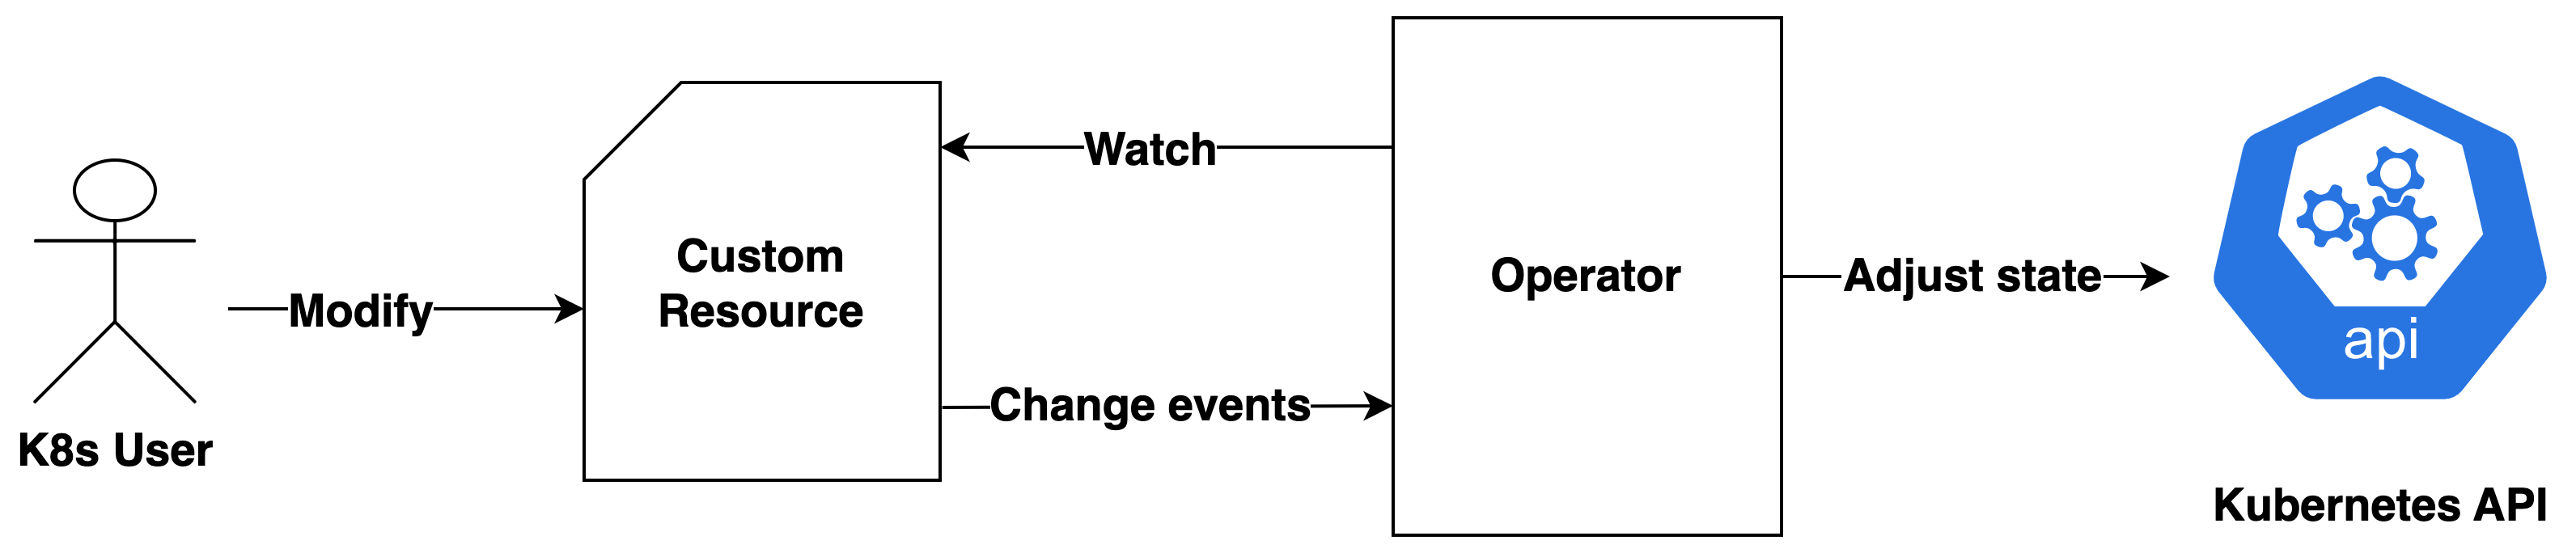
\includegraphics[width=1\linewidth]{images/opeartor_paradigm.png}
    \caption{Operator paradigm}
    \label{fig:operator_paradigm}
\end{figure}

\subsection{Helm}

Helm is a package manager for Kubernetes. Therefore with Helm it is possible to define, install and manage Kubernetes applications in a simpler way compared to a manual management of Kubernetes resources manifests \cite{helm}.
Helm is a graduated project in the CNCF and it is the de-facto standard for Kubernetes package management.
The key concept is the \textbf{Helm chart}, which is a collection of files that describe a related set of Kubernetes resources. 
These files are mainly of two types: templates and values.
The \textbf{templates} are Kubernetes manifest files that are rendered by Helm's \textbf{powerful templating engine}. 
The \textbf{values} are the set of variables that are used to render the templates.
Upon an Helm chart installation, Helm will render the templates ``injecting" the values and deploy the resources in the Kubernetes cluster.
One major advantage that Helm provides is the complete management of the lifecycle of the resources.
As a matter of fact, Helm allows to easily \textbf{upgrade}, \textbf{rollback} and \textbf{uninstall} the Kubernetes resources deployed with a Helm chart reducing time and errors in such operations \cite{helm}. 
Without Helm, the user would have to deal with each single Kubernetes resource manifest file and manually apply changes to them.
Finally, users can benefit of Helm charts already developed by the community and leverage chart distribution within their organization using Helm repositories.

\section{Krateo PlatformOps}
\label{sec:krateo}

Krateo PlatformOps (Krateo) is an \textbf{open-source Kubernetes-based platform} that aims to provide a unified interface for managing any desired resource on any infrastructure \cite{krateo_docs}.
Krateo runs as a Kubernetes deployment inside a Kubernetes cluster but \textbf{acts as a control plane} even for resource external to the Kubernetes cluster.
The only requirement for this management is that the resources need to be logically descriptible using a YAML file which represents the desired state of the resources \cite{krateo_docs}.
% Platform engineering
% Developer platform: a unified environment providing tools, services, and infrastructure that enables teams to efficiently build, test, and deploy software without managing underlying complexity. This complexity is handled by the platform team.
% Recognized by Gartner. Gartner said ... by 2025 companies without a ... (cite)
Krateo is composed of three main parts:
\begin{itemize}[itemsep=0.2pt, topsep=1pt]
    \item[$\bullet$] Krateo Composable Operations
    \item[$\bullet$] Krateo Composable Portal
    \item[$\bullet$] Krateo Composable FinOps
\end{itemize}

For the purpose of this work, we will focus on the \textbf{Krateo Composable Operations} part, which is the core of the Krateo platform and is responsible for managing the lifecycle of resources in a Kubernetes cluster \cite{krateo_docs}.
Krateo Composable Operations is composed in turn by several components. Due to their core importance in our system, as described in section XYZ we will briefly describe the functionalities of the \textbf{Krateo core-provider} and the \textbf{Krateo composition-dynamic-controller}.

\subsection{Krateo core-provider}

The Krateo core-provider is a Kubernetes operator that has the duty of downloading and managing Helm charts. It first checks for the existence of a file named \textit{values.schema.json} in the chart folder and uses it to generate a Kubernetes Custom Resource Definition (CRD), accurately representing the possible values that can be expressed for the installation of the chart \cite{krateo_core_provider}.
The file \textit{values.schema.json} is a JSON schema that describes the structure of the \textit{values.yaml} file for the related Helm chart and it is considered a standard best practice for Helm charts. It basically provides a way to validate the \textit{values}.yaml file before the Helm chart is installed (i.e., to check if the values are in the correct format).
In other words, the Krateo core-provider operator is responsible for deploying the Helm chart as a \textbf{native Kubernetes resource}, which allows for the management of the Helm chart lifecycle through Kubernetes APIs \cite{krateo_docs}.
As a matter of fact, out of the box, Kubernetes does not provide a way to manage Helm charts natively and the Krateo core-provider is one tool that allows to do so.
The Kubernetes Custom Resource Definition introduced by the Krateo core-provider is called \textbf{\textit{CompositionDefinition}}. It is a CRD that represents the Helm chart and its values (a Helm Chart archive (.tgz) with a JSON Schema for the values.yaml file) \cite{krateo_core_provider}.
Upon a CompositionDefinition manifest application to the Kubernetes cluster, the Krateo core-provider generates the CRD from the schema defined in the \textit{values.schema.json} file included in the chart. It then deploys an instance of the Krateo composition-dynamic-controller, setting it up to manage resources of the type defined by the CRD \cite{krateo_core_provider}.

\subsection{Krateo composition-dynamic-controller}

The Krateo composition-dynamic-controller is the Kubernetes operator that is instantiated by the Krateo core-provider to manage the Custom Resources whose Custom Resource Definition is generated by the core-provider.
In practice, when a Custom Resource (CR) is created, the instance of composition-dynamic-controller checks if a Helm release associated with the CR already exists in the cluster \cite{krateo_composition_dynamic_controller}. 
If this is not the case, it performs an \textit{helm install} operation using the values specified in the CR to create a new Helm release. This will practically deploy all the resources defined in the Helm chart using \textbf{Helm's templating engine}.
However, if the Helm release does already exist, it instead executes an \textit{helm upgrade} operation, updating the release's values with those specified in the CR, effectively updating the resources in the cluster.
Finally, when the CR is deleted from the cluster, the instance of the composition-dynamic-controller performs an \textit{helm uninstall} on the release, removing all the resources defined in the Helm chart from the cluster \cite{krateo_composition_dynamic_controller}. \\

The architecture of the Krateo core-provider and composition-dynamic-controller is depicted in Figure \ref{fig:krateo_core_provider}.

\begin{figure}[htb]
    \centering
    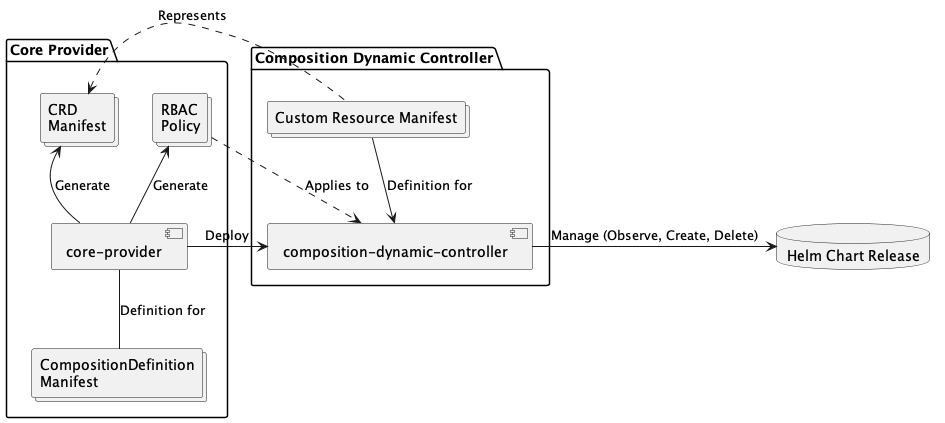
\includegraphics[width=1\linewidth]{images/kraeto_core_provider.png}
    \caption{Krateo core-provider and composition-dynamic-controller architecture \cite{krateo_core_provider}}
    \label{fig:krateo_core_provider}
\end{figure}

\section{Carbon-aware systems for resource management}

An analysis of existing systems have been made in order to...

\subsection{CASPER}

CASPER (Carbon-Aware Scheduling and Provisioning for Distributed Web Services) is a carbon-aware scheduling and provisioning system whose primary purpose is to minimize the carbon footprint of distributed web services \cite{Souza_2023}.
The system is defined as a multi-objective optimization problem that considers two factors: the \textbf{variable carbon intensity} and the \textbf{latency constraints} of the network \cite{Souza_2023}.
By evaluating the framework in real-world scenarios, the authors demonstrate that CASPER achieves significant reductions in carbon emissions (up to 70\%) while meeting application \textbf{Service Level Objectives (SLOs)}, highlighting its potential for practical implementation in large-scale distributed systems \cite{Souza_2023}.
The authors of CASPER highlight the importance of considering the workload characteristics such as memory state, latency and \textbf{regulatory constraints such as GDPR} \cite{Souza_2023}.


[HOW is it deployed]



\subsection{CASPIAN}

most important ptobably




\subsection{Let'sWaitAwhile}

test





\subsection{Other systems}

carbonScaler




\subsection{SOTA Recap}

many simulation, no real system
no much flexibility



usually either time shifting or geographical shifting
like letaswaitawhile is time shifting


\newpage
